\section{Fondamenti su LLM}
Un Large Language Model (LLM) è una rete neurale di grandi dimensioni addestrata su enormi quantità di testo per comprendere e generare linguaggio naturale. Gli LLM sono progettati per generare, riassumere, tradurre e analizzare testo in diversi contesti. Questo li rende la base tecnologica dietro ai moderni chatbot e assistenti virtuali \cite{Definizione_LLM}.

\subsection{Cos'è un LLM e il concetto di Large}
Tipicamente, con il termine \textit{large Language Models} (LLMs) ci si riferisce a modelli di linguaggio basati su architetture Transformer che contengono miliardi di parametri o più, i quali sono addestrati su quantità di testo massivo, come per GPT-3, PaLM, Galactica e LLaMA. Gli LLM hanno dimostrato avere forti capacità nel comprendere il linguaggio naturale e risolvere compiti complessi tramite generazione testuale.

Attualmente gli LLM sono principalmente costruiti sulla base dell'architettura Transformer, dove i layer di attenzione sono impilati in una rete neurale molto profonda.
Il concetto di Large negli LLM non presenta una definizione accademica rigorosa, ma si riferisce fondamentalmente ad un drastico salto di ordine di grandezza (scaling) sotto tre dimensioni principali:

\begin{itemize}
    \item \textbf{Numero di parametri:} i parametri sono i pesi (weights) e i bias della rete neurale, ovvero i valori numerici che il modello aggiorna durante la fase di apprendimento. Il termine Large entra in gioco con il passaggio da milioni di parametri a miliardi. I primi modelli pre-addestrati presentavano tra i 110 e i 340 milioni di parametri, mentre modelli come GPT-3 ne contano circa 175 miliardi.
    \item \textbf{Le dimensioni del dataset:} per evitare casi di overfitting addestrando modelli con miliardi di parametri, è necessario addestrarli su dataset di dimensioni enormi, che contengono centinaia di miliardi di token. Questi dataset sono spesso raccolti da fonti web, libri, articoli e altri tipi di testo. La dimensione del dataset è un fattore chiave per garantire che il modello possa generalizzare bene e non semplicemente memorizzare i dati di addestramento.
    \item \textbf{Le risorse computazionali:} anche le risorse computazionali necessarie per addestrare i modelli composti da molteplici GPU che lavorano in parallelo per un tempo esteso contribuiscono alla definizione di Large. L'addestramento di modelli con miliardi di parametri richiede infrastrutture di calcolo avanzate, come cluster di GPU o TPU, e può richiedere settimane o mesi per completare l'addestramento.
\end{itemize}

\subsection{L'evoluzione negli anni}
Negli ultimi anni, gli LLM hanno subito un'evoluzione significativa, passando da modelli relativamente piccoli a modelli con miliardi di parametri. Questa crescita ha portato a miglioramenti nelle capacità di comprensione e generazione del linguaggio, ma ha anche introdotto nuove sfide in termini di sicurezza e vulnerabilità.
Tecnicamente, la modellazione del linguaggio (LM) rappresenta uno dei principali approcci per far progredire l'intelligenza linguistica delle macchine. In generale, un modello di linguaggio mira a modellare la probabilità generativa di sequenze di parole, così da predire le probabilità dei token futuri.
La ricerca sui modelli di linguaggio ha ricevuto molte attenzioni nella letteratura, tanto da poter essere divisa in quattro periodi principali di sviluppo \cite{surveylargelanguagemodels} :
\begin{itemize}
    \item \textbf{Statistical language models (SLM):} sono stati sviluppati negli anni '90 basandosi su metodi di apprendimento statistico. L'idea era quella di modellare la predizione delle parole basandosi sulle assunzioni di Markov, predicendo la prossima parola sfruttando il contesto più recente. Questi modelli, sono stati ampiamente utilizzati per migliorare le prestazioni in Information Retrieval (IR) e in Natural Language Processing (NLP).
    Tuttavia questi modelli soffrono spesso di problemi legati alla dimensionalità: è difficile stimare accuratamente modelli di linguaggio di ordine elevato, poiché è necessario stimare un numero esponenziale di probabilità di transizione.
    \item \textbf{Neural language models (NLM):} i modelli di linguaggio neurali (NLM) modellano la probabilità delle sequenze di parole attraverso l'uso di reti neurali, come ad esempio il perceptron multistrato (MLP) e le reti neurali ricorrenti (RNN). Un notevole contributo è quello di aver introdotto il concetto di rappresentazione distribuita (distributed representation) delle parole e aver costruito la funzione di predizione della parola condizionata dalle caratteristiche aggregate del contesto.
    In seguito, word2vec ha introdotto un nuovo approccio per la costruzione di una rete neurale shallow, ovvero a un solo hidden layer, per imparare le rappresentazioni distribuite delle parole, migliorando così l'efficienza tra una varietà di attività NLP. Questi studi hanno iniziato l'uso dei language models per il representation learning, avendo quindi un importante impatto nel campo dell'NLP.
    \item \textbf{Pre-trained language model (PLM):} Come primo tentativo, ELMo è stato proposto per catturare rappresentazioni delle parole dinamiche e sensibili al contesto (context-aware), effettuando prima il pre-addestramento (pre-training) di una rete LSTM bidirezionale (biLSTM) invece di apprendere rappresentazioni fisse delle parole e successivamente il fine-tuning della rete biLSTM su specifici task a valle (downstream task). Inoltre, basandosi sull'architettura Transformer, che è altamente parallelizzabile e dotata di meccanismi di self-attention, è stato proposto BERT, il quale pre-addestra modelli di linguaggio bidirezionali tramite task di pre-addestramento appositamente progettati su corpora di grandi dimensioni e non etichettati. Queste rappresentazioni contestuali e pre-addestrate delle parole si rivelano molto efficaci come feature semantiche di uso generale, innalzando notevolmente gli standard prestazionali nei task di NLP. Questo studio ha ispirato un gran numero di lavori successivi, stabilendo il paradigma di apprendimento basato su "pre-training e fine-tuning". Seguendo questo paradigma, è stato sviluppato un elevato numero di studi sui modelli di linguaggio pre-addestrati (PLM), che hanno introdotto architetture differenti (es. GPT-2 e BART) oppure strategie di pre-addestramento migliorate. In tale paradigma, è spesso necessario effettuare il fine-tuning del PLM per adattarlo ai diversi downstream task.
    \item \textbf{Large Language Models (LLM):} I ricercatori osservarono che lo scaling dei Pre-trained Language Models (PLM) porta spesso a una migliore capacità del modello nei downstream task.
    Sebbene lo scaling venga applicato principalmente alle dimensioni del modello, mantenendo architetture e task di pre-addestramento simili, questi PLM di grandi dimensioni mostrano comportamenti differenti rispetto ai PLM più piccoli (ad es., BERT da 330 milioni di parametri e GPT-2 da 1,5 miliardi di parametri) e rivelano abilità sorprendenti nella risoluzione di una serie di task complessi. Ad esempio, GPT-3 è in grado di risolvere task few-shot attraverso l'apprendimento nel contesto (in-context learning), mentre GPT-2 non ottiene buoni risultati. Di conseguenza, la comunità scientifica ha coniato il termine 'modelli di linguaggio di grandi dimensioni (LLM)' per questi PLM su larga scala, i quali stanno attirando una crescente attenzione da parte della ricerca.
\end{itemize}

Il concetto di modello di linguaggio non è una novità tecnica specifica degli LLM, ma si è evoluto nel corso dei decenni di pari passo con i progressi dell'intelligenza artificiale. I primi modelli di linguaggio miravano principalmente a modellare e generare dati testuali, mentre i modelli di linguaggio più recenti, ad esempio GPT-4, si concentrano sulla risoluzione di task complessi. Questo passaggio, dalla modellazione del linguaggio alla risoluzione di task, rappresenta un importante salto nel pensiero scientifico, che costituisce la chiave per comprendere lo sviluppo dei modelli di linguaggio nella storia della ricerca.
Il concetto stesso di "Large" si è evoluto attraverso l'architettura Mixtrue of Experts (MoE): durante la generazione di un singolo token, un meccanismo di routing attiva solo una piccola frazione dei parametri totali del modello, consentendo così di scalare a modelli con trilioni di parametri senza aumentare proporzionalmente i costi computazionali. 

\subsection{L'architettura di un Transformer e il Meccanismo di Attenzione} 
L'architettura Transformer è stata introdotta da Vaswani et al. nel 2017 nel paper \textit{Attention is All You Need} \cite{attention_is_all_you_need} ed è stata la chiave di volta per lo sviluppo dei modelli di linguaggio di grandi dimensioni.
Nel paper originale viene presentata un'architettura composta da un encoder e un decoder \ref{fig:Transformer}: l'encoder mappa una sequenza di simboli in input $(x_1, ..., x_n)$ in una rappresentazione continua $z = (z_1, ..., z_n)$. Dato $z$ il decoder genera un output  $y_1,..., y_m$ come una sequenza di simboli, un elemento alla volta. Il decoder è auto-regressivo, ovvero predice il token successivo basandosi sui token precedenti, consumando i simboli generati precedentemente come input addizionale per quello successivo.

\begin{figure}[H]
    \centering
    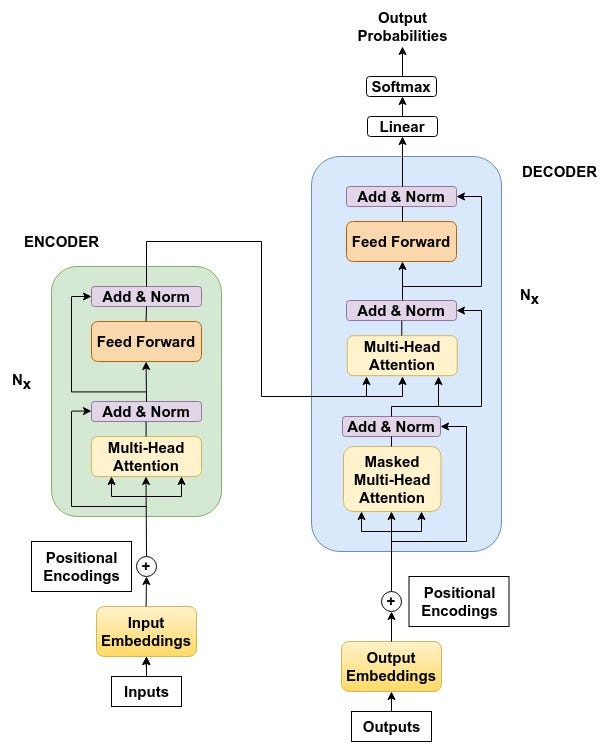
\includegraphics[width=0.45\textwidth]{immagini/encoder_decoder.jpg}
    \caption{L'architettura di un Transformer Encoder-Decoder.}
    \label{fig:Transformer}
\end{figure}

Sebbene il Transformer originale fosse basato su un'architettura bidirezionale di tipo Encoder-Decoder, i modelli linguistici moderni utilizzano un approccio di tipo Decoder-only, eliminando completamente l'Encoder e utilizzando solo il Decoder.
Non esiste quindi più una separazione netta tra "fase di lettura" e "fase di scrittura": il modello considera l'input iniziale, il prompt, e la risposta del modello stesso come un'unica grande sequenza di testo continuo.

Il Decoder è composto da più strati sequenziali, chiamati layer. 
Rispetto all'architettura originale del 2017,oggi ogni layer del Transformer è composto da soli due sottostrati (sub-layer): la Self-Attention e una rete Feed-Forward (FFN) che utilizza funzioni di attivazione come SwiGLU o GeLU; versioni più efficienti rispetto alla vecchia ReLU proposta nel paper originale.
Anche il flusso interno dei dati ha subìto un'ottimizzazione: oggi si preferisce normalizzare l'input prima che entri nei sub-layer (approccio Pre-LN), utilizzando varianti più snelle e veloci da calcolare come la RMSNorm (Root Mean Square Normalization), che sostituisce la standard Layer Normalization.
C'è però un aspetto cruciale che è rimasto intatto dal 2017 a oggi: il mascheramento causale (causal masking). Questo meccanismo impedisce rigorosamente all'algoritmo di "guardare nel futuro", garantendo che il modello, sia in fase di addestramento che di generazione vera e propria, impari a predire il token successivo basandosi esclusivamente su quelli che lo precedono.

\begin{figure}[H]
    \centering
    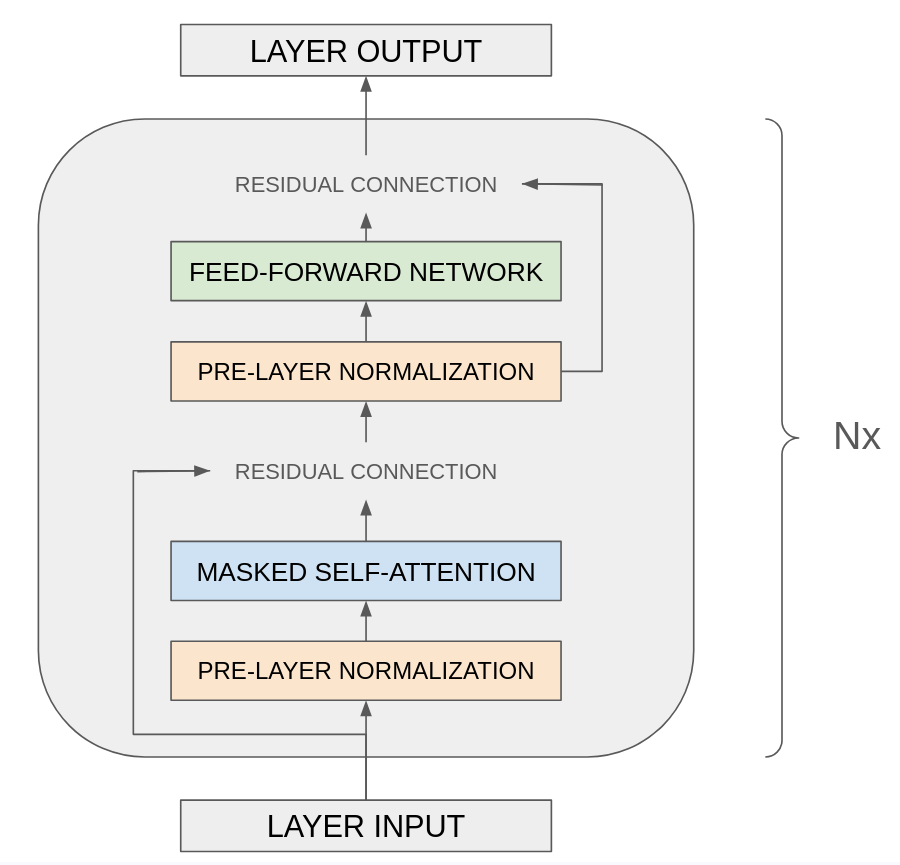
\includegraphics[width=0.45\textwidth]{immagini/decoder_only.png}
    \caption{L'architettura di un Transformer Decoder-only.}
    \label{fig:Transformer-DecoderOnly}
\end{figure}

Al fine di comprendere il funzionamento di un LLM, è fondamentale esporre l'architettura dei layer del decoder.
Per migliorare la stabilità di training viene utilizzato un layer di \textbf{pre-normalizzazione}: l'input viene normalizzato per ogni sub-layer del transformer invece di normalizzare l'output. Possono essere utilizzate diverse tecniche di normalizzazione come la RMSNorm.
Le funzioni di attivazioni tipicamente adottate sono la SwiGLU (Swish-Gated Linear Unit) o la GeLU: in particolar modo la SwiGLU ha una curva matematica che non azzera in modo netto i valori negativi, ma li attenua gradualmente e attraverso l'uso di gate decide quali informazioni lasciare passare. \cite{LLama_layer}

Il meccanismo di attenzione è il cuore dell'architettura Transformer. Esso consente al modello di pesare dinamicamente l'importanza di diverse parti dell'input quando genera una risposta. Nello specifico, la self-attention permette al modello di considerare tutte le parole in una frase o in un contesto più ampio, assegnando loro pesi diversi a seconda della loro rilevanza per il compito specifico. In particolar modo la funzione di attenzione può essere descritta come una mappatura di una query e un set di coppie chiave-valore ad un output, dove la query, le chiavi, valori e output sono tutti vettori. L'output è quindi calcolato come una somma pesata dei valori, dove il peso assegnato ad ogni valore è calcolato applicando una funzione di compatibilità della query con la chiave corrispondente.

Nel dettaglio ci si riferisce all'attenzione con il nome di \textbf{Scaled Dot-Product Attention}, dove l'input è formato dalle query e dalle chiavi di dimensione $d_k$, e dai valori di dimensione $d_v$, dove con $d$ ci si riferisce alla dimensione dei vettori. Viene calcolato il prodotto scalare tra le query con tutte le chiave, ciascuno diviso per $\sqrt{d_k}$, e applicando una funzione softmax per ottenere i pesi sui valori.

Un altro aspetto fondamentale dei transformer è l'attenzione multi-testa (multi-head attention), che consente al modello di prestare attenzione congiuntamente a diversi sottospazi di rappresentazione in diverse posizioni. In questo modo, il modello può catturare diversi tipi di relazioni tra le parole e i concetti.
Questo meccanismo può essere suddiviso in tre fasi:
\begin{enumerate}
\item \textbf{Proiezione e sdoppiamento:} le matrici di Query, Key e Value vengono proiettate linearmente per $h$ volte, dove $h$ è il numero di teste di attenzione, creando così $h$ versioni diverse e compatte delle query, chiavi e valori. Ognuna di queste versioni rappresenta una "testa" (head) di attenzione.
\item \textbf{Calcolo in parallelo:} viene calcolata in parallelo la Scaled Dot-Product su ciascuna delle $h$ teste.
\item \textbf{Concatenazione e output}: gli $h$ risultati ottenuti vengono concatenati tra loro e moltiplicati per un'ultima matrice di pesi, generando i valori dell'output finale.  
\end{enumerate}

La multi-head attention nel decoder permette ad ogni posizione nel decoder di prestare attenzione a tutte le posizioni precedenti fino a quella posizione. Bisogna prevenire l'information flow da posizioni future, per preservare la proprietà auto-regressiva del modello. Per questo motivo, viene applicato un mascheramento causale (causal masking) durante lo scaled dot-product attention impostando a $-\infty$ i valori delle connessioni illegali prima di applicare la funzione softmax.

\subsection{Rappresentazioni Vettoriali e Spazio Latente}
Gli LLM rappresentano il testo in uno spazio vettoriale ad alta dimensione, noto come spazio latente. In questo spazio, le parole, le frasi e i concetti sono rappresentati come vettori numerici, che catturano le relazioni semantiche tra di essi. Ad esempio, parole con significati simili tendono ad essere rappresentate da vettori vicini nello spazio latente, mentre parole con significati diversi sono rappresentate da vettori più distanti. Questa rappresentazione consente al modello di comprendere e generare testo in modo più efficace, poiché può sfruttare le relazioni semantiche tra le parole per produrre risposte coerenti e pertinenti.

Il primo passo per poter introdurre il concetto di rappresentazioni vettoriali è quello di definire il concetto di token: l'unità fondamentale di testo che un modello di linguaggio elabora.
Questo è una sequenza di caratteri che può rappresentare una parola, una parte di parola o anche un carattere singolo a seconda del contesto.

Per poter generare un token vengono utilizzati algoritmi come \textbf{Byte Pair Encoding (BPE)}, una tecnica di compressione dati che iterativamente rimpiazza le coppie di byte più frequenti in una sequenza con un singolo byte inutilizzato. Nel contesto dei modelli di linguaggio, BPE viene utilizzato per suddividere il testo in token, dove, invece di unire le coppie di bytes più frequenti, vengono uniti caratteri o sequenze di caratteri.
Viene inizializzato il simbolo del vocabolario con i caratteri individuali, viene poi rappresentata ogni parola come una sequenza di caratteri ed un simbolo speciale di fine parola, il quale permette di ripristinare la parola originale. Successivamente vengono contate le coppie di simboli e ogni occorrenza della coppia più frequente viene sostituita con un nuovo simbolo.
Ogni operazione di merge produce un nuovo simbolo che rappresenta un $n$-gramma di caratteri.
Il nuovo token viene quindi aggiunto al vocabolario ed il processo di conteggio e fusione viene ripetuto iterativamente, espandendo il vocabolario con nuovi token sempre più lunghi.
L'algoritmo termina quando viene raggiunta la dimensione del vocabolario prefissata.\cite{sennrich2016neuralmachinetranslationrare}
Per ovviare ai limiti del BPE, la ricerca si sta spostando verso architetture Token-Free o Byte-Level, rendendo i modelli nativamente multilingue.

Strettamente collegato al concetto di token c'è quello di embedding: ovvero vettori di numeri reali che codificano il significato di un oggetto in un formato che può essere elaborato da un modello di machine learning. Formalmente è il risultato di una funzione $f: X \rightarrow \mathbb{R}^n$ che mappa uno spazio discreto $X$, come parole, documenti o immagini, in uno spazio vettoriale continuo di dimensione $n$, preservando relazioni semantiche come distanza e direzione. \cite{cosa_sono_gli_embeddings} 
Il flusso per generare gli embedding inizia con la tokenizzazione del testo fornito al modello, che suddivide il testo in token.
Vengono poi recuperati gli embeddings contestualizzati per ogni token ed infine attraverso Attention e media pesata viene generato un embedding complessivo che rappresenta l'intero input testuale.

Proprietà chiave degli embeddings è che oggetti semanticamente simili sono rappresentati da vettori vicini nello spazio latente.\cite{mikolov2013efficientestimationwordrepresentations}

Esistono diversi tipi di embeddings, caratterizzati per il tipo di oggetto rappresentato possiamo distinguere: word, sentence e document, image e graph embeddings.
I primi sono associati a singole parole, sentence e document rappresentano intere frasi o documenti con un singolo vettore, gli image sono il risultato di reti convoluzionali o vision transformer mentre i graph rappresentano nodi di un grafo.

Nello stadio iniziale del training di un LLM, i vettori che rappresentano le parole sono casuali o frutto di un pre-inizializzazione.  Il modello, durante la fase di training analizza ingenti quantità di testo così da osservare diversi contesti.
Tramite questo processo iterativo, i valori numerici all'interno dei vettori vengono progressivamente aggiornati e raffinati: i vettori che rappresentano parole con significati o funzioni affini finiscono per posizionarsi vicini nello spazio geometrico ad alta dimensionalità, catturando e rendendo così esplicite le relazioni semantiche e sintattiche del linguaggio.

Se l'Embedding è la partenza, gli Hidden States rappresentano le mutazioni del vettore dopo che è stato creato nella Matrice di Embedding.
Formalmente, l'Hidden State è l'attivazione della rete, ovvero la rappresentazione vettoriale di un token in un dato layer all'interno del modello.
L'architettura moderna è descritta attorno al concetto di \textbf{Residual Stream}.\cite{elhage2021mathematical}\\
Il Residual Stream è il flusso di dati che attraversa i layer del modello, è possibile riassumere il processo per ogni layer come segue:
\begin{enumerate}
    \item Il primo Hidden State contiene solo il significato base del vocabolario
    \item Viene quindi applicata la Self-Attention, che consente al modello di leggere l'Hidden State corrente e quello dei token precedenti.
    \item Viene così generato e sommato al precedente vettore un nuovo vettore, così da aggiornare l'Hidden State
    \item Subito dopo, la rete Feed-Forward legge il vettore appena modificato e lo elabora ulteriormente, generando un nuovo vettore che viene sommato al precedente, aggiornando così nuovamente l'Hidden State.
\end{enumerate}

Questo ciclo di lettura e scrittura si ripete in modo identico per tutti i layer successivi, aggiornando e arricchendo progressivamente la complesittà semantica dell'Hidden State fino all'output finale.

Ogni vettore viene mappato in uno spazio vettoriale chiamato anche Hidden Space o Spazio Latente: uno spazio geometrico ad alta dimensionalità in cui i vettori rappresentano concetti, parole o frasi. Esso costituisce, di fatto, la mappa concettuale che permette al modello di codificare e manipolare le relazioni logiche e di significato del linguaggio.
